\chapter{\MakeUppercase{Шагающие роботы}}

\section{Задачи работы}

В рамках работы рассматривается разработка шагающего четырехногого робота, с упором на проблему разработки конечностей и программирования.

Для выполнения работы требуется:
\begin{itemize}
    \item Рассчитать худший (по нагрузке) статический случай для конечностей 4-х ногого робота.
    \item Подобрать электроприводы удовлетворяющие по крутящему моменту.
    \item Подобрать остальные комплектующие, входящие в состав робота и обеспечивающие его автоновную работу.
    \item Спроектировать и собрать физическую модель робота.
    \item Запрограммировать управление робота.
    \item Изучить управляемость и механические характеристики такого робота.
\end{itemize}

\section{Актуальность работы}

Задача разработки конечностей для шагающих роботов настолько же важная, как и задача навигации роботов. Сегодня она актуальна, как никогда ранее. Всё в большей степени людей стараются заменять шагающими роботами для работ, в которых требуется мобильность и подвижность человеческих ног, и при этом невозможно присутствие самого человека. Речь о работах вроде общего тех. осмотра помещений, исследования местности вдали от дорог и цивилизации, помощи в устранении последствий катастроф, пребывание в опасной для человека среде (под поздействием вредных газов, излучения). Открытость методик, исходных кодов и готовых моделей в открытом доступе приведет к массовой разработке шагающих роботов не только крупными предприятиями, но и мелкими разработчиками.

\section{Анализ}

Для поставленных ранее задач можно сформировать последовательность действий для дальнейшей работы. Хотя изначально данных было недостаточно, исходя из опыта были сделаны некоторые предположения по требуемым габаритам конечностей робота и крутящим моментам двигателей, которые в последствии оказались верны.

Далее исходя из дополненных данных о длинах и моментах нужно лишь рассчитать ограничение на массу тела робота, после чего можно продолжать работу.

\subsection{Рассчёт худшего статического случая}

«Худшим» случаем называется такой, при котором одному или нескольким приводам нужно приложить максимальный момент для поворота звена конечности в нужную сторону.

Для того чтобы определить худший случай, нужно вообще определиться с кинематикой конечностей. После изучения существующих на рынке роботов, было решено применить в своей конструкции наиболее распрострененное решение. Оптимальной кинематикой можно считать конечность с 3 степенями свободы:

\begin{figure}[ht]
    \centering
    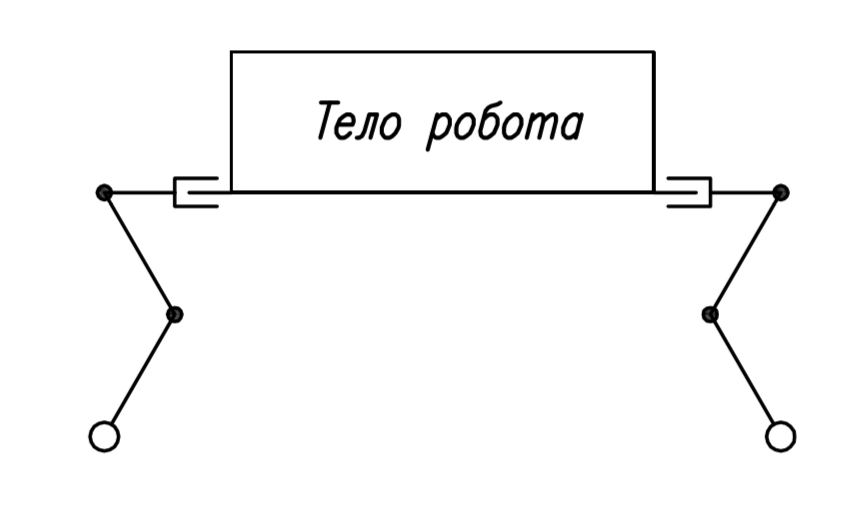
\includegraphics[scale=0.7]{kin1.png}
    \caption{Кинематика 4-х ногого робота, вид сбоку}
\end{figure}

Худшим случаем считается случай, в котором робот лежит на «животе» с выпрямленной конечностью. Чтобы подогнуть под себя конечность, нужно будет преодолеть момент $M_{худш}$ с учетом массы тела робота $m$. При этом максимальный крутящий момент потребуется приводу, находящемуся в первом узле, или можно сказать, управляющему первой степенью свободы.

\begin{figure}[ht]
    \centering
    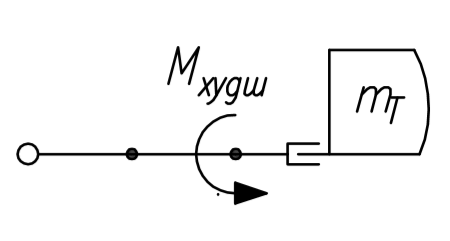
\includegraphics[scale=1]{kin2.png}
    \caption{Кинематика 4-х ногого робота, вид сбоку (худший случай)}
\end{figure}

При расчёте в первом приближении можно пренебречь трением и весами звеньев. Также можно учесть, что нагрузка, создаваемая массой тела робота будет распределена равномерно по всем 4-м ногам. Это значит что на одну ногу будет приходится лишь $\frac{1}{4}m$ тела робота.

Также, в первом приближении допустим, что тело робота может достигать 2-х килограмм. Большая часть веса придется на каркас конструкции, собранный из пластика. Меньшая часть веса придется на аккумулятор. Еще более маленькая часть придется на проводку и крепежи. Самыми легкими составляющими конструкции окажутся электронные компоненты.

При таком расчете можно считать что каждой ноге надо будет «поднять» около 0.25 кг веса. Тогда в худшем случае, приложенный момент вычисляется просто:
$$ M_{худш}= \frac 1 4 (l_{1}+l_{2}) m g, $$
\noindent здесь $l_1$ и $l_2$ - длины звеньев.

Мы можем подобрать длины звеньев таким образом, чтобы они обеспечивали достаточную для задач ходьбы рабочую область и одновременно наименьший требуемый момент.

Спроектированные для прототипа конечности имеют характеристики:
\begin{align*}
    l_1 &\approx (44 + 87) \times 10^{-3} = 131\: мм \\
    l_2 &\approx 134.5 \times 10^{-3} = 134.5\: мм
\end{align*}

\noindent С использованием приводов с крутящим моментом $ 2.5 \: Н $ максимально допустимый вес робота будет примерно равен $ 3.8 \: кг $. Такое требование к весу, с учетом изготовления деталей из аллюминия и пластика, вполне выполнимо.

После получения оценочных данных можно переходить к проектированию основных узлов робота.